  \subsubsection{Асимметричный случай отражения}
  Весьма наглядной иллюстрацией являются собственные кривые отражения от Si(440) рассчитанные при
  трех разных углах падения и соответсвенно имею разный коэффициент асимметрии. Угол
  Брегга для такой плоскости отражения составляет $\theta_B = 21.68^o$, угол наклона поверхности
  составляет $\varphi = 20^o 53^{'}$.

  \begin{figure}[H]
  \centering
  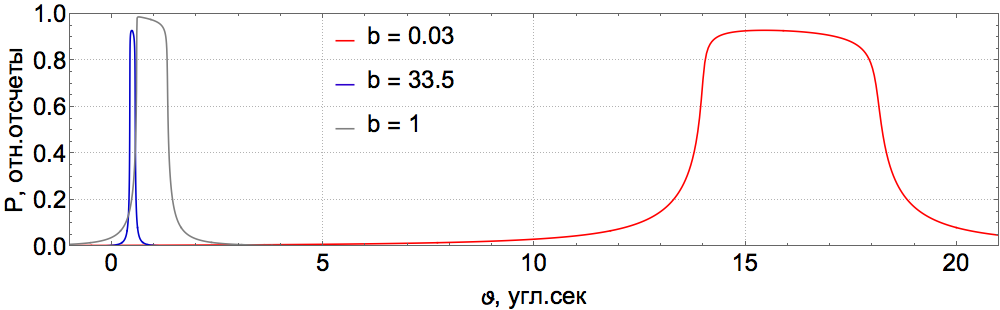
\includegraphics[width=0.99\textwidth]{images/rocking_curve_assym_3.png}
  \caption{Кривые отражения 440 $MoK_{\alpha 1}$ от Si, полученные при разных углах падения(для разных b)}
  \label{ris:rocking_curve_assym_3}
  \end{figure}
  Сдвиг центра кривой происходит из-за наличия преломления на величину 0.5 и 16.5 угловых секунд.

  Варьируя угол между поверхностью кристалла и отражающей плоскостью (например, с помощью шлифовки),
  можно существенно изменить ширину рентгеновского пучка (рисунок ~\ref{ris:assym_width_beam}).
  \begin{figure}[H]
   \centering
   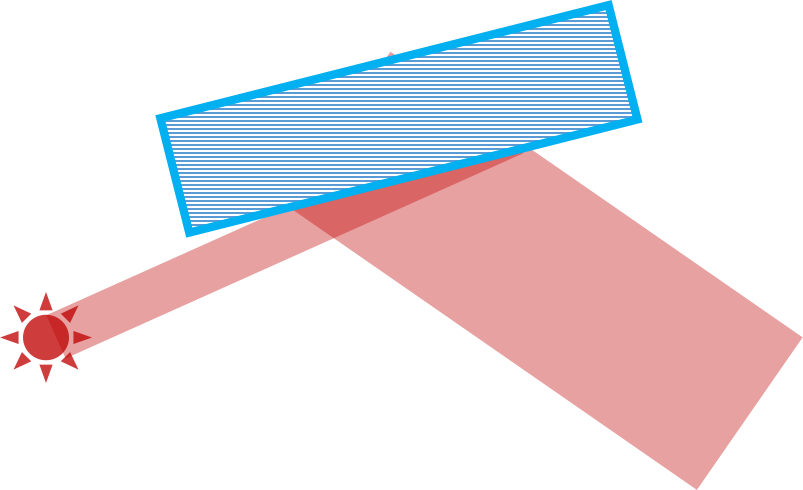
\includegraphics[width=0.4\textwidth]{images/assym_width_beam.png}
   \caption{Кристалл с асимметричным отражением по Бреггу}
   \label{ris:assym_width_beam}
  \end{figure}


  \begin{figure}[H]
    \centering
    \subfloat[$b = 33.52$, $\varphi$ > 0]{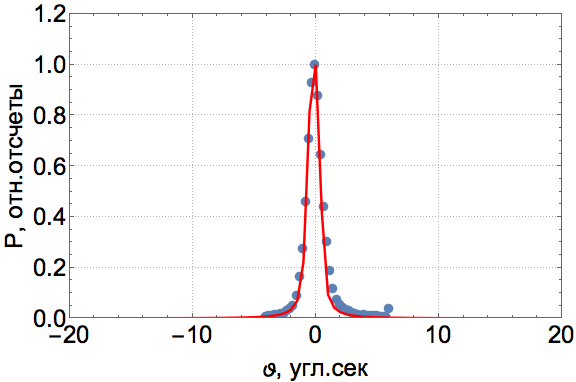
\includegraphics[width=0.45\textwidth]{images/assym-blue-50.png}}
    \hfill
    \subfloat[$b = 0.03$, $\varphi$ < 0]{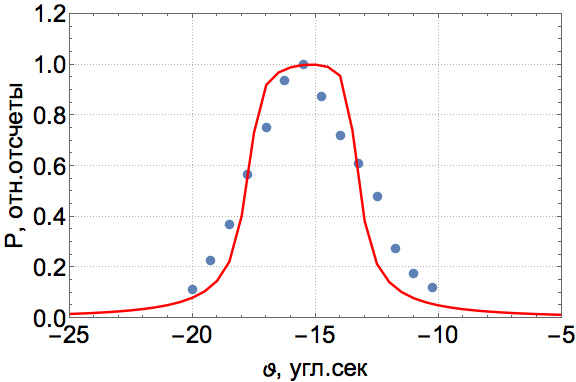
\includegraphics[width=0.45\textwidth]{images/assym-red-50.png}}
    \caption{Двухкристальная КДО для схемы с кристаллом монохроматором Si(440) и асимметричным образцом Si(440),
    угол разориентации поверхности $\varphi = 20^o53^{'}$. Размер щелевых устройств $S_1 = S_2 = 50$ мкм.}
    \label{ris:assymetric_exp_50}
  \end{figure}
